% 内点の図：集合 O の中の点 a と、その周りの開球体
%
% ビルド: bash figures/build.sh
% 出力先: content/set-topology/from-euclidean-to-topology-interior-point.svg
%
% 本文の右に横並びで置く小さめの図。縦長にしてある。
% 生成されるSVGは黒の線画で固定（ダークモードでも白地の上に表示する）。

\documentclass[uplatex,dvipdfmx,border=4pt,varwidth]{standalone}
\usepackage{plautopatch}
\usepackage{amsmath,amssymb}
\usepackage{tikz}

\begin{document}
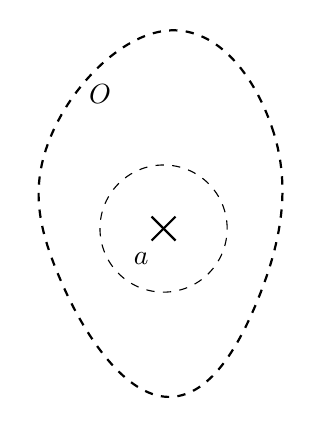
\begin{tikzpicture}[scale=0.95]
  % 集合 O（いびつな縦長の閉曲線）
  \draw[dashed, thick] plot[smooth cycle, tension=0.75]
    coordinates {(0.1,3.0) (1.45,1.7) (1.3,-0.5) (0.05,-1.9) (-1.35,-0.4) (-1.5,1.6)};

  % 開球体 B^{(n)}(a; varepsilon)
  \draw[dashed] (0,0.35) circle (0.85);

  % 点 a（バツ印）
  \draw[thick] (-0.16,0.19) -- (0.16,0.51);
  \draw[thick] (0.16,0.19) -- (-0.16,0.51);

  % ラベル
  \node at (-0.85,2.15) {$O$};
  \node at (-0.3,-0.05) {$a$};
\end{tikzpicture}
\end{document}
